\documentclass[11pt, oneside]{article}   	% use "amsart" instead of "article" for AMSLaTeX format
\usepackage{geometry}                		% See geometry.pdf to learn the layout options. There are lots.
\geometry{letterpaper}                   		% ... or a4paper or a5paper or ... 
%\geometry{landscape}                		% Activate for rotated page geometry
%\usepackage[parfill]{parskip}    		% Activate to begin paragraphs with an empty line rather than an indent
\usepackage{graphicx}				% Use pdf, png, jpg, or eps§ with pdflatex; use eps in DVI mode
								% TeX will automatically convert eps --> pdf in pdflatex		
\usepackage{amssymb}

%SetFonts

%SetFonts


\title{Modeling explosive percolation on directed networks}
\author{Shannon Moran}
\date{PHYS 514, Fall 2017}							% Activate to display a given date or no date

\begin{document}
\maketitle

\section{Motivation}

For my final project, I was particularly motivated by taking what we'd learned and applying it to a problem recently discussed in the literature. Part of the value I see in graduate courses is that they provide you with the vocabulary to go out and understand related literature without studying the exact problems in class.

The paper I chose to investigate was ``Explosive percolation on directed networks due to monotonic flow of activity'', published in PRE by the D'Souza and Lu groups in July 2017 \cite{Waagen_2017}. In this paper, the authors looked to replicate the observed growth of tweets in response to the discovery of the Higgs boson (this data set is publicly available as part of the Stanford Large Network Dataset Collection, hence the interest). These authors saw the growth of the tweet network and recognized it as \textbf{explosive percolation}.

Explosive percolation  is said to occur in an evolving network when a macroscopic connected component emerges in a number of steps that is much smaller than the system size, and there have  been a number of papers (e.g. \cite{Achlioptas_2009}) that have explored this phenomena in random networks.

I particularly liked this paper because it took topics that we had covered in class and extended them, as shown in Figure \label{fig:classwork}. I will detail the implementation of these processes in the Methods section, and discuss a few specific findings in the Results and Discussion section. Note that this brief report is also accompanied by a jupyter notebook of code examples, annotated code used in this project, and the presentation given on December 13.

\section{Methods}

\subsection{Percolation processes}

The percolation processes used in the paper are based on the Directed Erdos-Renyi (DER) proces, which is a stochastic, unbiased network generation algorithm. Here, the authors add in an order (ODER) and competition plus order (C-ODER) rule. These algorithms are summarized in Figure \ref{fig:perc-processes}.

Each network is characterize by $n$ nodes and $m$ edges. We can also combine these into a measure called ``edge density'', $\delta=\frac{m}{n}$. Each directed edge points from a \textit{tail} to a \textit{head}.

\subsection{Cluster definition and algorithms}
In lattice percolation, we're familiar with clusters defined as occupied sites connected to occupied nearest neighbor sites. In random network percolation, we refer to networks of nodes connected by edges as components. In percolation on directed networks, we study strongly connected components (SCCs). Nodes $a$ and $b$ are considered in the same SCC if $a$ can reach $b$ and $b$ can reach $a$ via directed edges.

This is illustrated below:\footnote{Source: https://commons.wikimedia.org/wiki/File:Scc.png} \\
\begin{center}
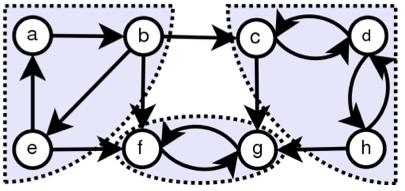
\includegraphics[scale = 0.5]{figs/SCC.png}
\end{center}

Algorithms for finding clusters tend to be highly problem-specific. While we used the Hoshen-Kopelman algorithm for lattices, and Newman-Ziff is used for undirected graphs, we use Tarjan's Algorithm for finding the SCCs of directed graphs \cite{Tarjan_1972}. This is a depth-first search. The order of operation is:
\begin{itemize}
\item Two parameters are tracked for each node, v
\begin{itemize}
\item v.index = time stamp at which vertex v is discovered
\item v.low = oldest ancestor v can reach
\end{itemize}
\item For each node:
\begin{itemize}
\item Add the node to the stack
\item For each child:
\begin{itemize}
\item If child has already been visited: recursively run the SCC-finding function, an set v.low = min of the node's low and the child's low
\item Elif child is in the current stack: v.low is the minimum of node's low and child's low
\item If v.low and v.index are equal, the stack down to the node is one SCC
\end{itemize}
\end{itemize}
\end{itemize}

Because of this recursion, I run into stack overflow issues and am unable to study networks with greater than \verb|n=1E3| nodes. Additional information, as well as an implementation using an open-source SCC-finding algorithm, is provided in the jupyter notebook.

\subsection{Critical exponents}

With their competitive, ordered process, the authors are interested in comparing their results with prior work on competitive percolation networks. In a 2011 \textit{Nature Physics} paper, Nagler et al demonstrated that the largest jump in the size of the largest component of a system would scale as $N^{-\beta}$ \cite{Nagler_2011}.

However, they find that ``the only exception seems to be global competition, where [they] find $\beta$ to be indistinguishable from zero''. That is precisely what Waagen et al find-- or claim to find-- for both the ODEr and C-ODER processes.

To study this, we must find the single link addition that generates the largest jump in the size of the largest SCC. Recalculating after the addition of every edge would be prohibitively computationally expensive. Instead, they build out the graph, tracking the order in which edges were added, then use a binary search on the completed graph to find the largest jump. With this process, the cost of the operation is only $O(E\log{E})$.

\section{Results and Discussion}

\subsection{Studying the growth of the largest SCC: Paper figures 5, 6, and 8}

As shown in Figure \ref{fig:fig56}, I am able to replicate the shapes of both the ODER and C-ODER curves of largest SCC size versus edge density, including a series of large jumps near the ``critical edge density'' ($\delta_c$) for the C-ODER study. However, my graphs are significantly shifted towards smaller edge densities, though when I increase the number of nodes by a factor of 10, they begin to shift to the right.

This immediately tells me that the $\delta_c$ is not system-size invariant. While the authors frame edge density as an analog to the probability $p$ of a site being occupied in lattice percolation, this is misleading. In lattice percolation, $p_c$ of there being a percolating cluster in the system is invariant to system size-- it is just the shape of the distribution that changes with system size (wider distribution for smaller systems, a step function for an infinite system).

Not to leave this stone unturned, I then looked for a variable that would capture the probability of a large cluster existing relative to the number of edges added, without varying with number of nodes. My most promising idea was to study the fraction of a system connected to an average node ($\frac{\delta}{n}$) rather than edge density. However, as is obvious from Figure \ref{fig:fig56-proposal}, this was a bust.

Finally, it is worth noting that this shift is not due to a failure in my implementation's ability to replicate the mechanisms of SCC formation. As shown in Figure \ref{fig:fig8}, I am able to replicate the mechanism of the largest SCC ``jump'' at the $\delta_c$ by the combination of the two largest SCCs.

\subsection{Studying the critical exponent: Paper figure 7}

As shown in Figure \ref{fig:fig7}, I am able to replicate the authors' finding that the critical exponent of the growth of the size of the largest cluster with system size appears to be zero. Even at my much smaller system sizes, I get a similar average size of ``largest jump'' relative to system size.

\section{Conclusions}
Not only did I learn about network theory in doing this project-- a field I hadn't studied before-- I also was able to use my understanding of the percolation methods we discussed in class to understand and then implement analogous methods in networks (rather than lattices).

\bibliographystyle{unsrt}
\bibliography{Bibliography}




\newpage

\begin{figure}[h]
\centering
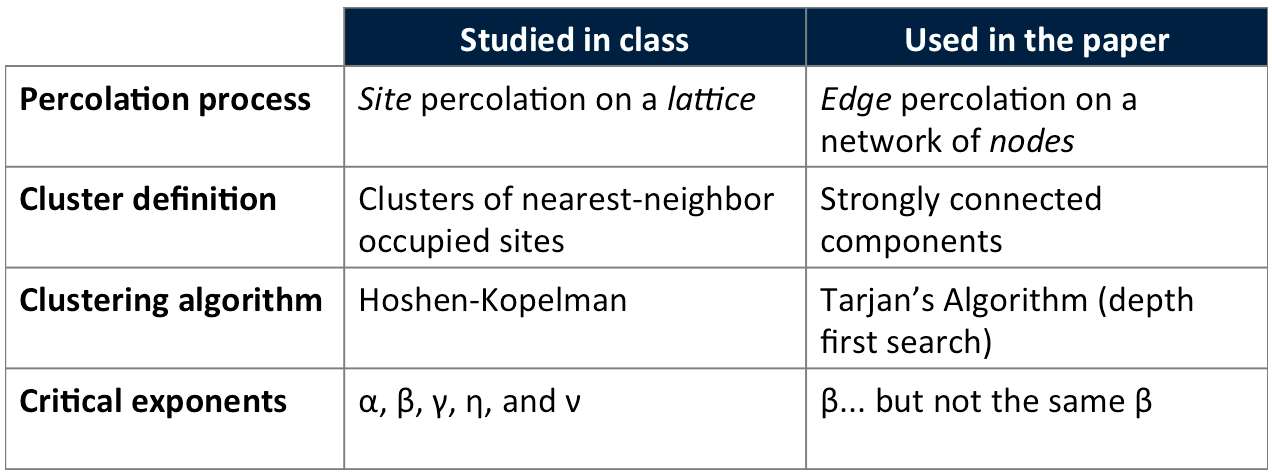
\includegraphics[width =\textwidth]{figs/classtopics.png}
\caption{Comparison of topics studied in class, versus those discussed in the paper by Waagen et al.}
\label{fig:classwork}
\end{figure}

\begin{figure}[h]
\centering
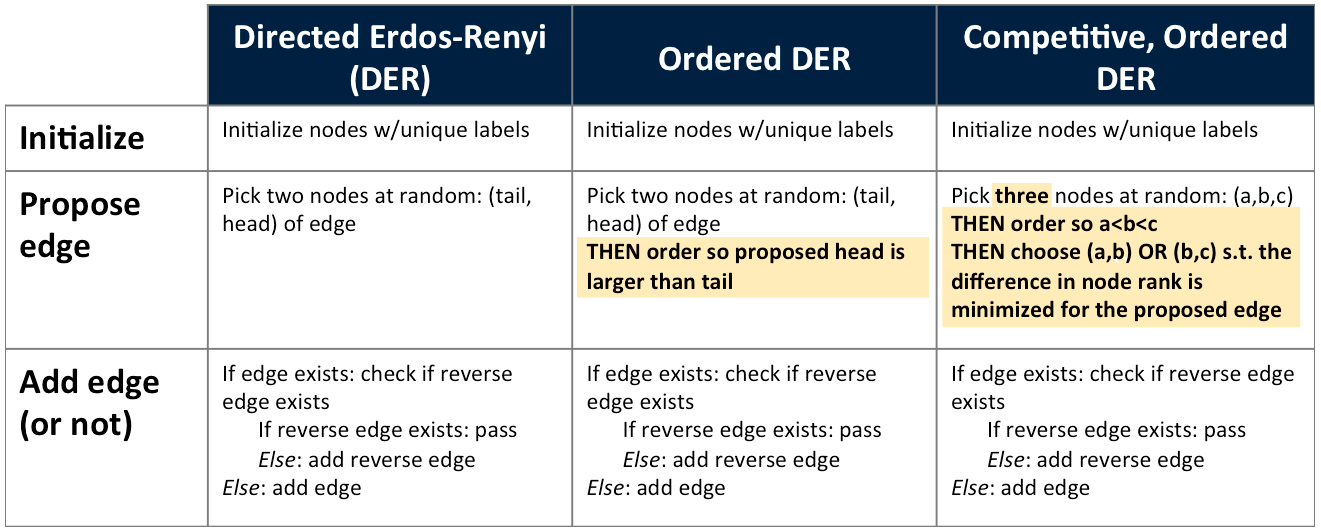
\includegraphics[width =\textwidth]{figs/perc-processes.png}
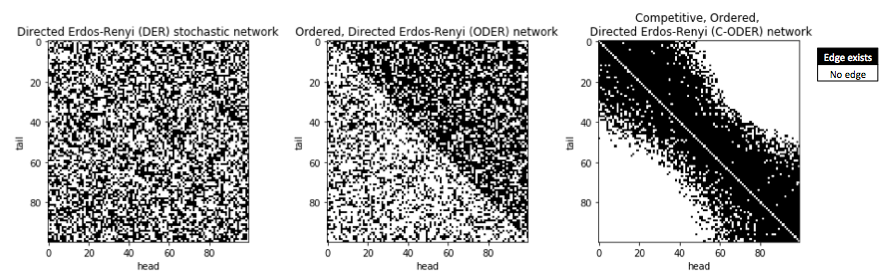
\includegraphics[width =\textwidth]{figs/percolation.png}
\caption{Explanation of percolation processes covered in Waagen et al., and the adjacency matrices resulting from their implementation.}
\label{fig:perc-processes}
\end{figure}

\begin{figure}[h]
\centering
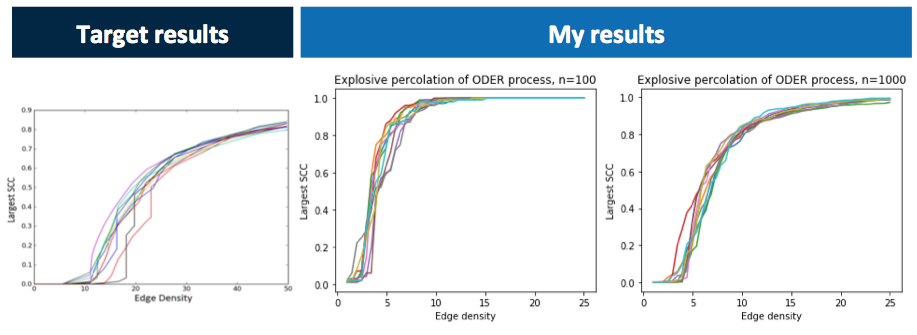
\includegraphics[width =\textwidth]{figs/fig5-oder.png}
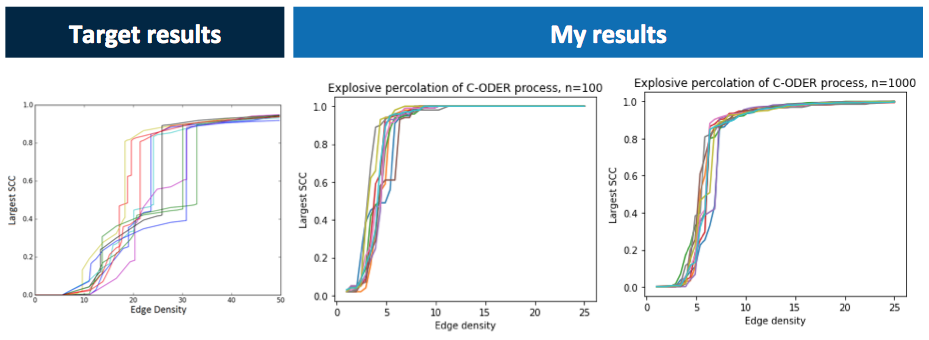
\includegraphics[width =\textwidth]{figs/fig6-coder.png}
\caption{Replication of Figures 5 (top, for the ODER process) and 6 (bottom, for the C-ODER process) from Waagen et al. Both the paper and my simulations were run for 10 replicates, though Waagen et al use a system size of n=1E6. My system sizes are as indicated.}
\label{fig:fig56}
\end{figure}


\begin{figure}[h]
\centering
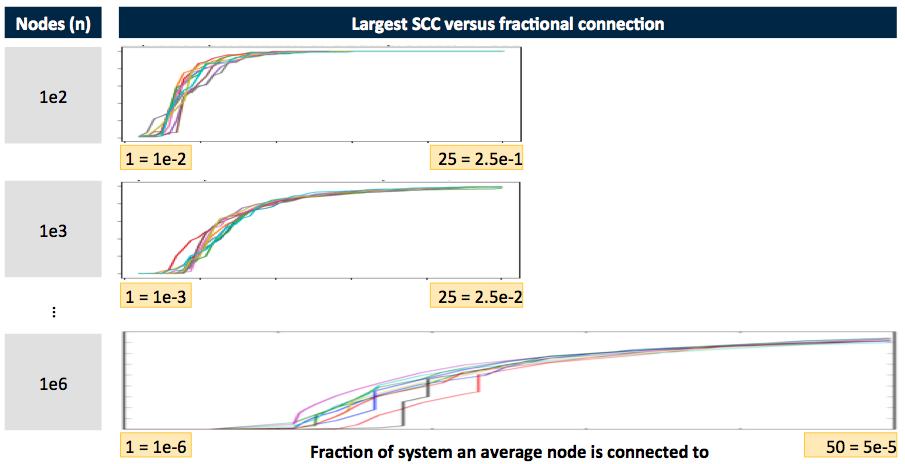
\includegraphics[width =\textwidth]{figs/fig56-proposal.png}
\caption{Illustration of using fraction of network connected to an average node, rather than edge density, as the x-coordinate.}
\label{fig:fig56-proposal}
\end{figure}


\begin{figure}[h]
\centering
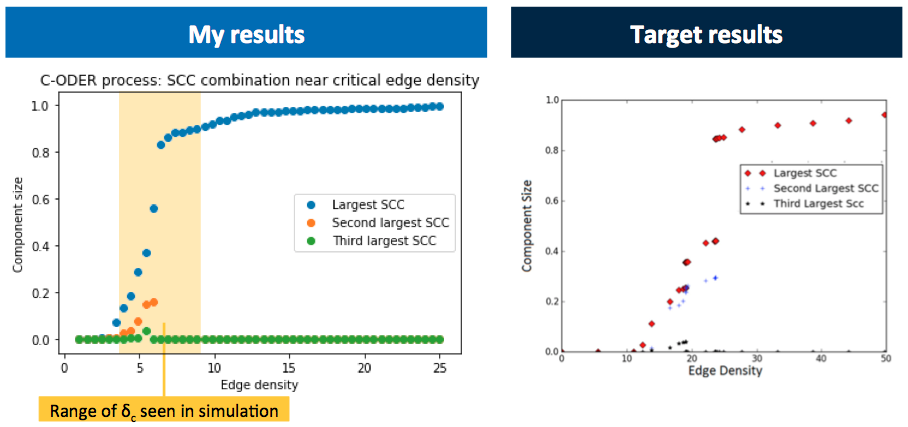
\includegraphics[width =\textwidth]{figs/fig8.png}
\caption{Replication of Figure 8 from Waagen et al. While the paper uses 1 replicate at a system size of n=1E6, I use 1 replicate at a system size of n=1E2.}
\label{fig:fig8}
\end{figure}


\begin{figure}[h]
\centering
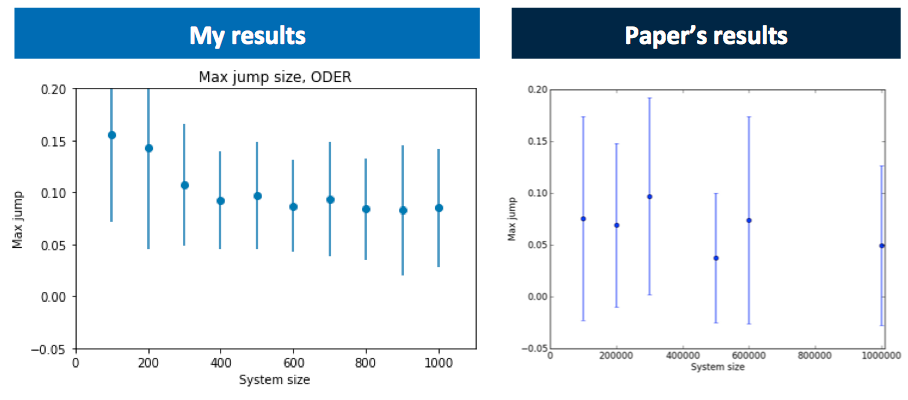
\includegraphics[width =\textwidth]{figs/fig7-oder.png}
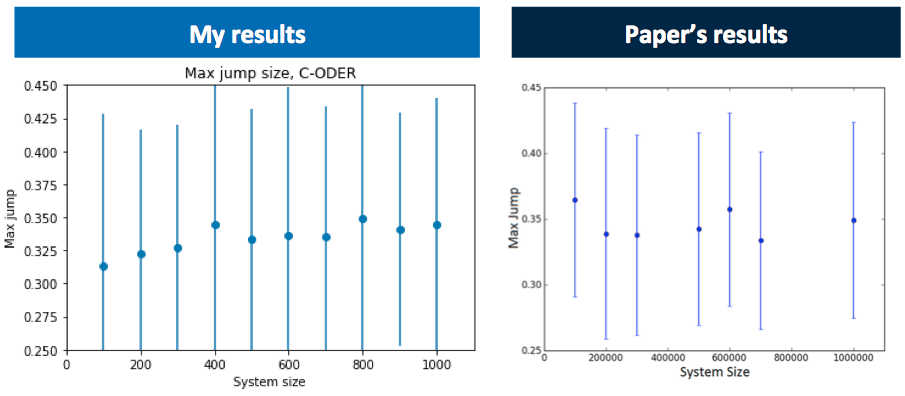
\includegraphics[width =\textwidth]{figs/fig7-coder.png}
\caption{Replication of Figure 7 from Waagen et al. Both the paper and my results represent the average and standard deviation of 40 replicates. I assumed an edge density of 50; the edge density used in the paper figures was not stated.}
\label{fig:fig7}
\end{figure}

\end{document} 